\section{软件开发环境}

\begin{itemize}
    \item \textbf{编程语言}:C++ \verb|20|
    \item \textbf{UI 开发框架}:Qt \verb|6.7.0|
    \item \textbf{数据库}:MySQL \verb|8.3.0|
    \item \textbf{IDE}:Qt Creator \verb|13.0.2|
    \item \textbf{系统}: macOS Sonoma \verb|14.5(23F79)|
\end{itemize}

\section{快速上手}

\begin{enumerate}
    \item 克隆仓库至本地,cd进入 \begin{cppcode}
              git clone https://github.com/Word2VecT/Pokemon.git
              cd Pokemon
          \end{cppcode}
    \item 安装对应版本的 Qt,并在 Qt Creator 中配置
    \item 安装 MySQL 数据库,并启动后台监听服务,程序使用数据库用户名为 root,密码为空, 数据库名为 Pokemon, 也可以自行修改 \cppinline{Server/main.cpp} 文件配置为本地
    \item 使用命令导入数据库 \begin{cppcode}
              mysql -u root -p < ./Database/Pokemon.sql
          \end{cppcode}
    \item 在 Qt Creator 中打开 \cppinline{Server} 项目,编译运行
    \item 在 Qt Creator 中打开 \cppinline{Client} 项目,编译运行
    \item Enjoy!
\end{enumerate}

\section{模块清单}
% Please add the following required packages to your document preamble:
% \usepackage{longtable}
% Note: It may be necessary to compile the document several times to get a multi-page table to line up properly
\begin{longtable}[c]{|c|c|c|}
    \caption{模块清单}                                         \\
    \hline
    \textbf{模块名称} & \textbf{模块标识符} & \textbf{模块说明}         \\ \hline
    \endfirsthead
    %
    \endhead
    %
    开始窗口          & MainWindow     & 开始界面                  \\ \hline
    登陆窗口          & LoginDialog    & 用于完成登陆、注册功能的窗口        \\ \hline
    游戏大厅          & Home           & 游戏大厅                  \\ \hline
    背包界面          & Bag            & 显示用户所有的Pokemon 及精灵选择  \\ \hline
    Pokemon 展示子项  & ListItem       & 在背包或选择中展示Pokemon 基础信息 \\ \hline
    Pokemon 信息界面  & pokemonInfo    & 显示Pokemon 的信息         \\ \hline
    用户列表          & Rank           & 显示所有用户的信息             \\ \hline
    对战选择          & Battle         & 显示对战种类选择              \\ \hline
    对战界面          & Stadium        & 显示对战过程                \\ \hline
    结果界面          & Result         & 显示对战结果                \\ \hline
\end{longtable}

\section{图形界面设计}

\begin{figure}[H]
    \centering
    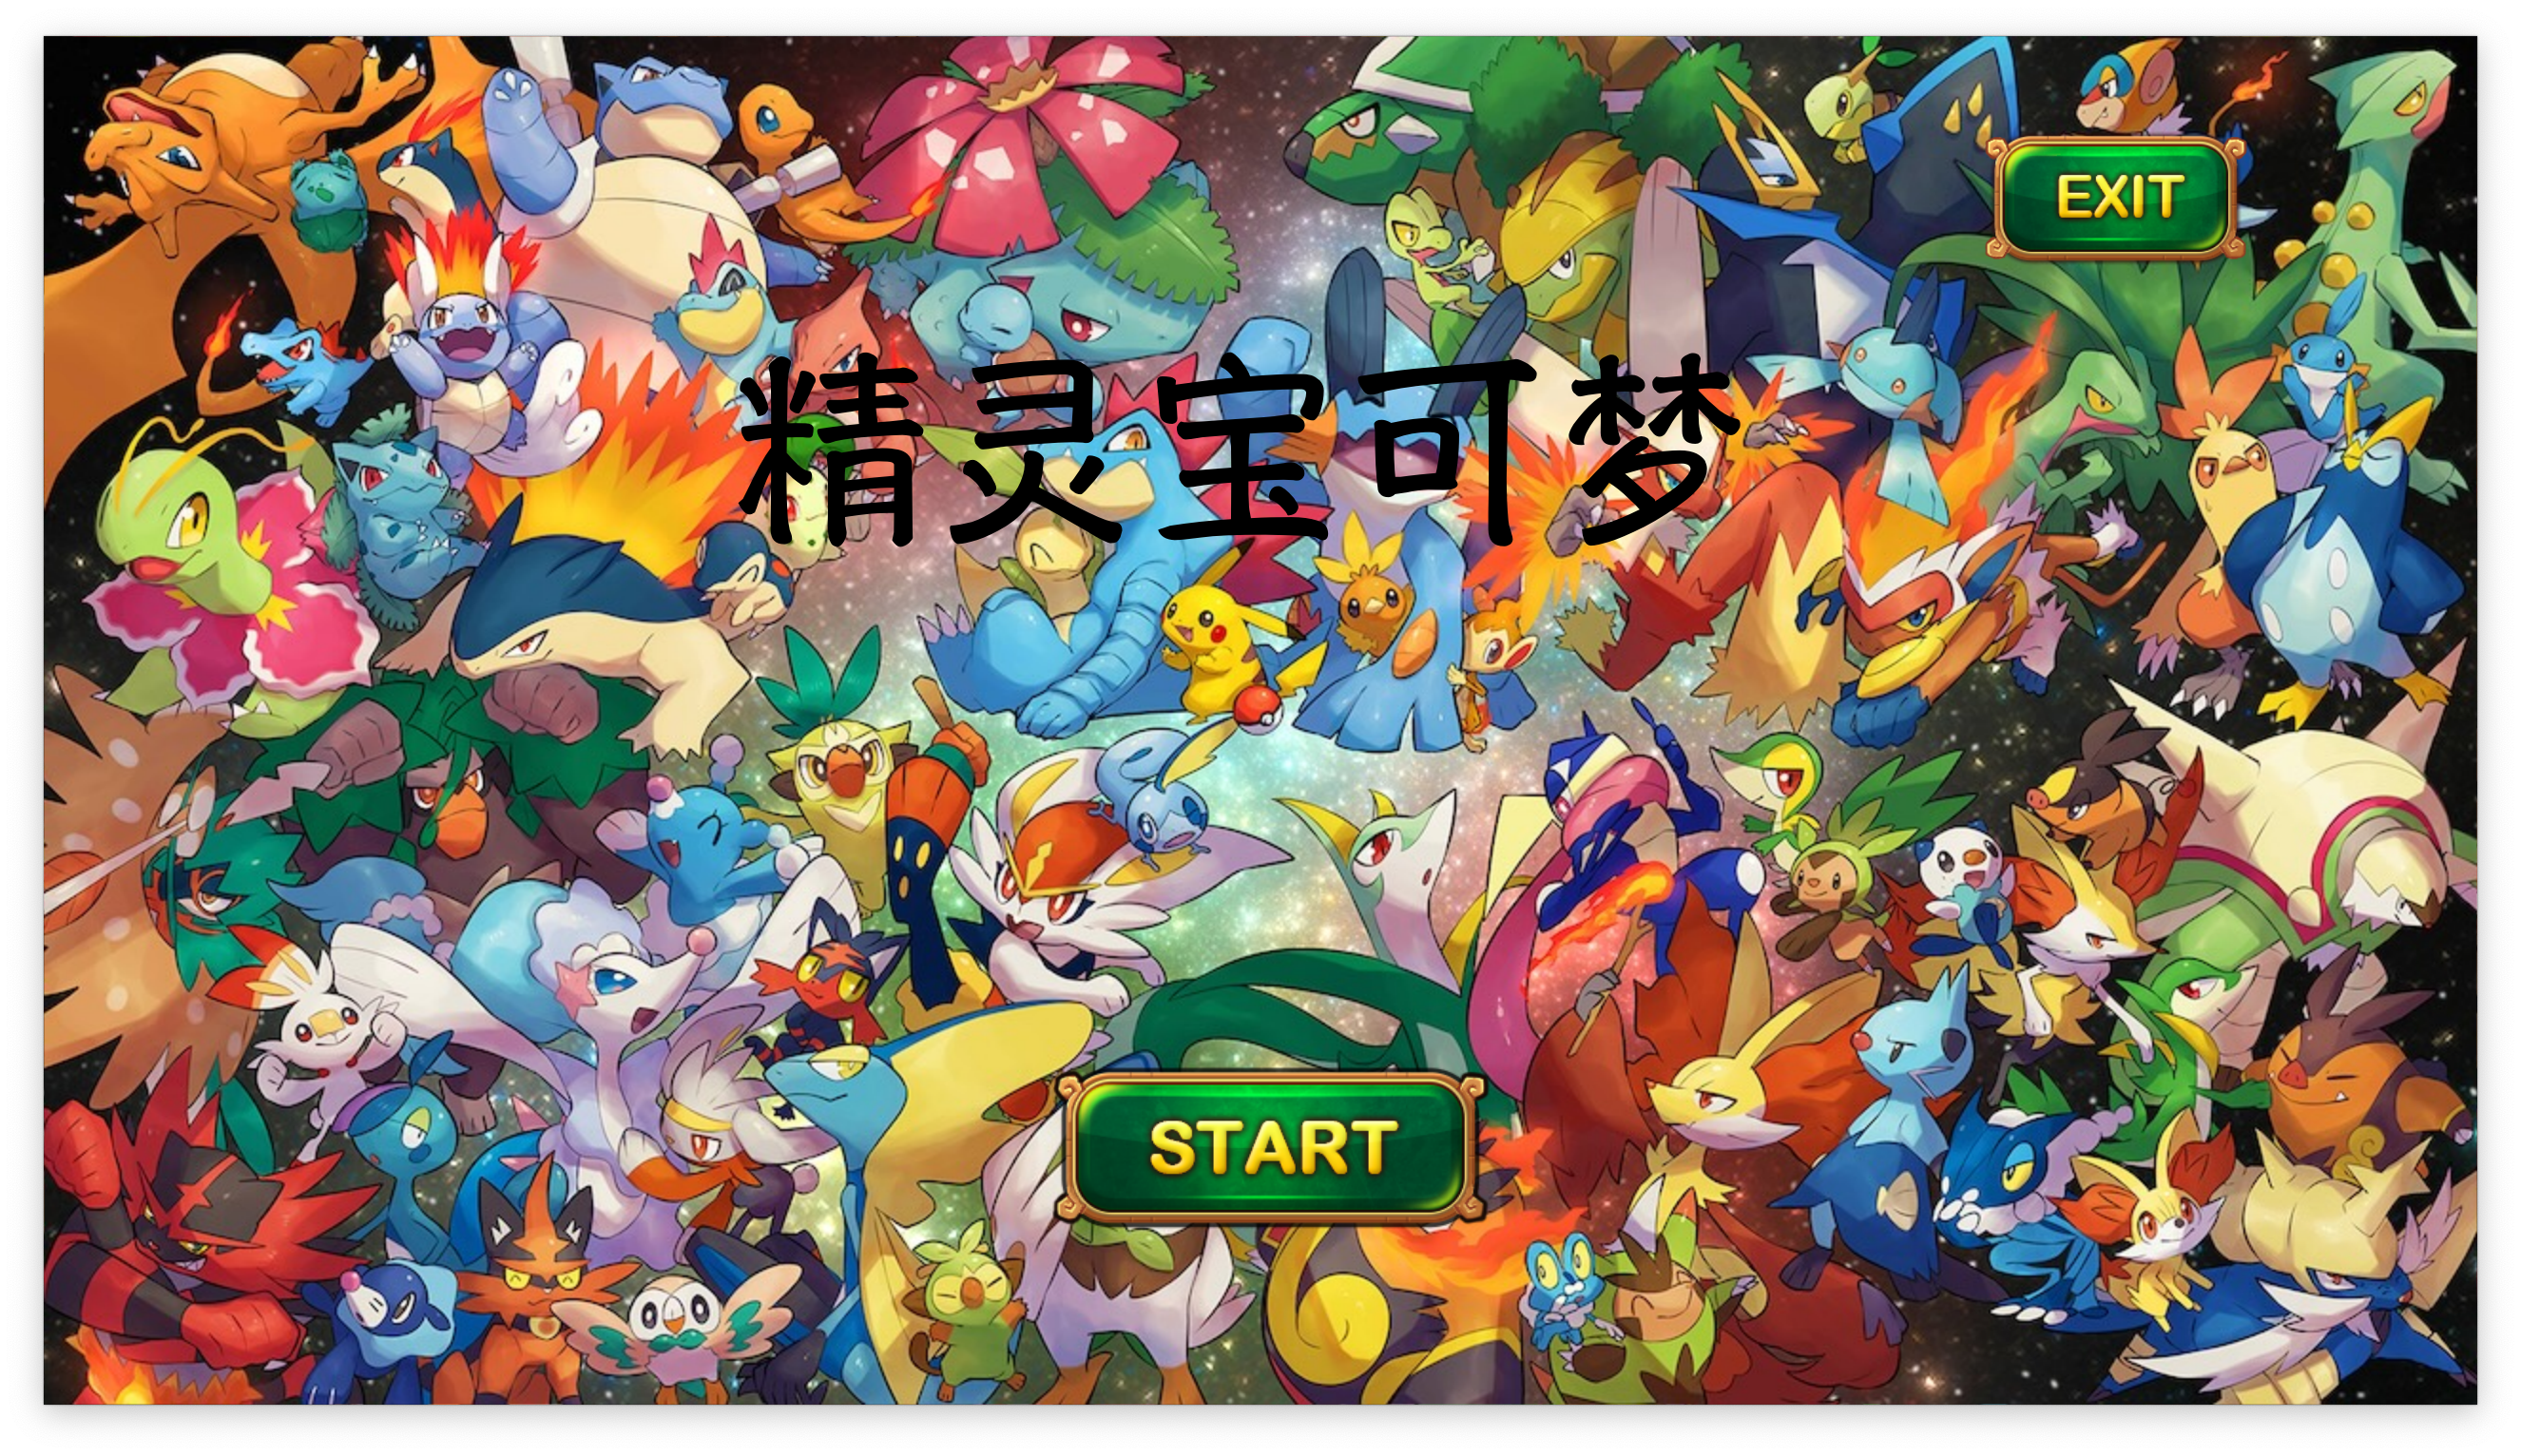
\includegraphics[width=0.8\textwidth]{main.png}
    \caption{开始界面}
\end{figure}

\begin{figure}[H]
    \centering
    \includegraphics[width=0.5\textwidth]{login.png}
    \caption{登录界面}
\end{figure}

\begin{figure}[H]
    \centering
    \includegraphics[width=0.8\textwidth]{home.png}
    \caption{游戏大厅}
\end{figure}

\begin{figure}[H]
    \centering
    \includegraphics[width=0.8\textwidth]{user.png}
    \caption{用户列表}
\end{figure}

\begin{figure}[H]
    \centering
    \includegraphics[width=0.6\textwidth]{info.png}
    \caption{用户信息}
\end{figure}

\begin{figure}[H]
    \centering
    \includegraphics[width=0.6\textwidth]{pokemon.png}
    \caption{Pokemon 信息界面}
\end{figure}

\begin{figure}[H]
    \centering
    \includegraphics[width=0.8\textwidth]{choose.png}
    \caption{对战选择界面}
\end{figure}

\begin{figure}[H]
    \centering
    \includegraphics[width=0.8\textwidth]{battle.png}
    \caption{对战界面}
\end{figure}


\begin{figure}[H]
    \centering
    \includegraphics[width=0.8\textwidth]{win.png}
    \caption{对战胜利界面}
\end{figure}

\begin{figure}[H]
    \centering
    \includegraphics[width=0.8\textwidth]{lose.png}
    \caption{对战失败界面}
\end{figure}

\section{宠物 Pokemon 类设计}

设计了宠物 Pokemon 的类, 模拟了精灵的各种属性和行为. 精灵的属性包括名字、等级、经验值、攻击力、防御力、生命值、速度、种类和能力. 每个精灵有独特的攻击方式, 等级提升时属性会相应增加. 为了方便扩展, 精灵的攻击方法设计为虚方法.

\subsection{类设计}

\subsubsection{基类:Pokemon}

\cppinline{Pokemon} 类是所有精灵的基类, 包含以下主要属性和方法:

\begin{itemize}
    \item 属性:\begin{itemize}
              \item \cppinline{id}:精灵的唯一标识符
              \item \cppinline{name}:精灵的名字
              \item \cppinline{lv}:精灵的等级
              \item \cppinline{exp}:精灵的经验值
              \item \cppinline{atk}:精灵的攻击力
              \item \cppinline{def}:精灵的防御力
              \item \cppinline{hp}:精灵的生命值
              \item \cppinline{speed}:精灵的速度
              \item \cppinline{type}:精灵的种类
              \item \cppinline{ability}:精灵的能力
          \end{itemize}
    \item 方法:\begin{itemize}
              \item 构造函数:初始化精灵的属性
              \item 各种 \cppinline{getter} 和 \cppinline{setter} 方法:获取和设置精灵的各个属性
              \item 虚函数 \cppinline{lvUp}: 精灵升级方法(派生类中实现)
              \item 虚函数 \cppinline{attack}: 精灵攻击方法(派生类中实现)
          \end{itemize}
\end{itemize}

\begin{cppcode}
    #ifndef POKEMON_H
    #define POKEMON_H

    #include <QString>
    #include "config.h"
    #include <QRandomGenerator>

    // 基类:Pokemon
    // 这个类表示一个基本的精灵, 包含了精灵的基本属性和方法
    class Pokemon {
            protected:
            int id; // 精灵的唯一标识符

            QString name; // 精灵的名字
            bool evolved; // 精灵是否已进化

            int lv; // 精灵的等级
            int exp; // 精灵的经验值

            int atk; // 精灵的攻击力
            int def; // 精灵的防御力
            int hp; // 精灵的生命值
            int speed; // 精灵的速度

            QString type; // 精灵的种类
            QString ability; // 精灵的能力

            public:
            // 构造函数, 初始化精灵的属性
            Pokemon(QString name = "", int lv = 1, int atk = INIT_ATK, int def = INIT_DEF, int hp = INIT_HP, int speed = INIT_SPEED, QString ability = "");

            // 虚析构函数
            virtual ~Pokemon() {};

            // 获取精灵的名字
            QString getName() const;
            // 获取精灵的唯一标识符
            int getID() const;
            // 获取精灵的等级
            int getLv() const;
            // 获取精灵的经验值
            int getExp() const;
            // 获取精灵的攻击力
            int getAtk() const;
            // 获取精灵的防御力
            int getDef() const;
            // 获取精灵的生命值
            int getHp() const;
            // 获取精灵的速度
            int getSpeed() const;
            // 获取精灵的能力
            QString getAbility() const;

            // 设置精灵的等级
            void setLv(int);
            // 设置精灵的经验值
            void setExp(int);
            // 设置精灵的攻击力
            void setAtk(int);
            // 设置精灵的防御力
            void setDef(int);
            // 设置精灵的生命值
            void setHp(int);
            // 设置精灵的速度
            void setSpeed(int);

            // 判断精灵是否死亡
            bool isDead() const;

            // 虚函数:精灵升级, 需要在派生类中实现
            virtual void lvUp() = 0;
            // 虚函数:精灵攻击另一个精灵, 需要在派生类中实现
            virtual int attack(Pokemon*) = 0;
        };

    #endif // POKEMON_H
\end{cppcode}

下面以力量型 Pokemon 为例, 说明 Pokemon 属性和方法的设计.

\subsubsection{派生类:AttackPokemon}

\cppinline{AttackPokemon} 类继承自 \cppinline{Pokemon} 类, 是可以攻击的精灵类. 在 \cppinline{AttackPokemon} 类中, 重写了 \cppinline{attack} 方法, 实现了精灵的攻击行为. 在攻击时, 精灵会根据自己的攻击力和对方的防御力计算伤害值, 然后对对方造成伤害.

\cppinline{lvUp}:精灵等级提升时, 属性增加, 如果精灵达到11级, 名字改变表示进化.

\begin{cppcode}
    #ifndef ATTACKPOKEMON_H
    #define ATTACKPOKEMON_H

    #include "pokemon.h"

    // 派生类:AttackPokemon
    // 这个类继承自Pokemon, 表示具有攻击能力的精灵
    class AttackPokemon : public Pokemon {
            public:
            // 继承基类Pokemon的构造函数
            using Pokemon::Pokemon;

            // 虚析构函数
            virtual ~AttackPokemon() {};

            // 重写基类的纯虚函数lvUp, 实现精灵升级的逻辑
            void lvUp() override;

            // 纯虚函数:精灵攻击另一个精灵, 需要在派生类中实现
            virtual int attack(Pokemon*) override = 0;
        };
\end{cppcode}

\subsubsection{派生类:Charmander}

\cppinline{Charmander} 类继承自 \cppinline{AttackPokemon}, 表示小火龙精灵. 重写了 \cppinline{attack} 方法, 定义小火龙的攻击逻辑:

\cppinline{attack}:计算攻击伤害并随机生成攻击效果, 如果小火龙等级大于10且触发灼烧效果, 额外增加伤害.

\begin{cppcode}
    Charmander::Charmander(QString name, int lv, int atk, int def, int hp, int speed) : AttackPokemon(name, lv, atk, def, hp, speed, "火花") {}

    int Charmander::attack(Pokemon* enemy) {
            int damage = atk - enemy->getDef();
            QRandomGenerator *generator = QRandomGenerator::global();
            int random = generator->bounded(6);
            if (random <= 2) {
                    damage *= random;
                }

            if (getLv() > 10 && generator->bounded(100) < getSpeed()) {
                    damage += 0.5 * getDef();
                } //灼烧效果
            enemy->setHp(fmax(enemy->getHp() - damage, 0));

            return random;
        }
\end{cppcode}

\subsubsection{派生类:Mankey}

\cppinline{Mankey} 类继承自 \cppinline{AttackPokemon}, 表示猴怪精灵. 重写了 \cppinline{attack} 方法, 定义猴怪的攻击逻辑:

\cppinline{attack}:计算攻击伤害并随机生成攻击效果, 如果猴怪等级大于10且触发防御降低效果, 降低敌方防御并增加自身攻击力.

\begin{cppcode}
    Mankey::Mankey(QString name, int lv, int atk, int def, int hp, int speed) : AttackPokemon(name, lv, atk, def, hp, speed, "踢倒") {}

    int Mankey::attack(Pokemon* enemy) {
            int damage = atk - enemy->getDef();
            QRandomGenerator *generator = QRandomGenerator::global();
            int random = generator->bounded(6);
            if (random <= 2) {
                    damage *= random;
                }

            if (getLv() > 10 && generator->bounded(100) < getSpeed()) {
                    enemy->setDef(enemy->getDef() - 0.5 * getAtk());
                    setAtk(getAtk() + 0.5 * enemy->getDef());
                }//降低敌方防御

            enemy->setHp(fmax(enemy->getHp() - damage, 0));
            return random;
        }
\end{cppcode}

\subsection{测试程序}

\begin{cppcode}
    #include <QCoreApplication>
    #include "pokemon.h"
    #include "attackpokemon.h"
    #include <iostream>

    void printPokemonStats(const Pokemon& pokemon) {
            std::cout << "Name: " << pokemon.getName().toStdString() << std::endl;
            std::cout << "Level: " << pokemon.getLv() << std::endl;
            std::cout << "Attack: " << pokemon.getAtk() << std::endl;
            std::cout << "Defense: " << pokemon.getDef() << std::endl;
            std::cout << "HP: " << pokemon.getHp() << std::endl;
            std::cout << "Speed: " << pokemon.getSpeed() << std::endl;
            std::cout << "Ability: " << pokemon.getAbility().toStdString() << std::endl;
            std::cout << "Is Dead: " << (pokemon.isDead() ? "Yes" : "No") << std::endl;
        }

    int main(int argc, char *argv[])
    {
            QCoreApplication a(argc, argv);

            // Create some Pokemon instances
            Charmander charmander("Charmander", 5, 52, 43, 39, 65);
            Mankey mankey("Mankey", 5, 80, 35, 40, 70);

            // Print initial stats
            std::cout << "Initial Stats of Charmander:" << std::endl;
            printPokemonStats(charmander);

            std::cout << "\nInitial Stats of Mankey:" << std::endl;
            printPokemonStats(mankey);

            // Attack each other
            std::cout << "\nCharmander attacks Mankey!" << std::endl;
            charmander.attack(&mankey);
            printPokemonStats(mankey);

            std::cout << "\nMankey attacks Charmander!" << std::endl;
            mankey.attack(&charmander);
            printPokemonStats(charmander);

            // Level up Charmander
            std::cout << "\nCharmander levels up!" << std::endl;
            charmander.lvUp();
            printPokemonStats(charmander);

            // Level up Mankey
            std::cout << "\nMankey levels up!" << std::endl;
            mankey.lvUp();
            printPokemonStats(mankey);

            return 0;

            return a.exec();
        }
\end{cppcode}

\subsection{总结}

通过上述设计, 精灵类的继承和多态性得到了良好的体现. 每种精灵都有其独特的属性和攻击方式, 且可以在此基础上进一步扩展新的精灵种类和攻击逻辑. 通过测试程序, 可以验证各个类及其方法的正确性, 确保精灵在游戏中的行为符合设计预期.

\section{数据库设计}

\subsection{用户表 user}

% Please add the following required packages to your document preamble:
% \usepackage{longtable}
% Note: It may be necessary to compile the document several times to get a multi-page table to line up properly
\begin{longtable}[c]{|c|c|}
    \caption{用户表 user}           \\
    \hline
    \textbf{表项}    & \textbf{含义} \\ \hline
    \endfirsthead
    %
    \endhead
    %
    userID         & 用户ID        \\ \hline
    username       & 用户名         \\ \hline
    password       & 密码          \\ \hline
    online         & 在线状态        \\ \hline
    pokemonCnt     & 宝可梦数量       \\ \hline
    highPokemonCnt & 高级宝可梦数量     \\ \hline
    battleCnt      & 战斗次数        \\ \hline
    battleWinCnt   & 战斗胜利次数      \\ \hline
\end{longtable}

\subsection{宝可梦表 pokemon}

% Please add the following required packages to your document preamble:
% \usepackage{longtable}
% Note: It may be necessary to compile the document several times to get a multi-page table to line up properly
\begin{longtable}[c]{|c|c|}
    \caption{宝可梦表 pokemon}    \\
    \hline
    \textbf{表项} & \textbf{含义} \\ \hline
    \endfirsthead
    %
    \endhead
    %
    pokemonID   & 宝可梦 ID      \\ \hline
    name        & 名称          \\ \hline
    HP          & 生命值         \\ \hline
    ATK         & 攻击力         \\ \hline
    DEF         & 防御力         \\ \hline
    LV          & 等级          \\ \hline
    Speed       & 速度          \\ \hline
    userID      & 主人用户ID      \\ \hline
\end{longtable}

\section{界面设计}

Qt 的使用也体现了面向对象的编程思想:\begin{itemize}
    \item \textbf{类和对象}:Qt广泛使用类和对象来封装数据和功能. 每个控件、窗口、对话框等都被封装成类, 通过实例化类来创建对象, 这些对象负责管理自身的状态和行为.

          \textbf{继承}:Qt 利用继承机制来扩展和定制现有的类. 通过继承, 可以创建新的类并添加或修改功能, 而不需要从头开始编写代码. Qt 中许多控件都是从 \cppinline{QWidget} 或 \cppinline{QAbstractItemModel} 等基类继承而来的.

          \textbf{多态性}:Qt 通过虚函数和接口实现多态性, 使得程序可以在运行时选择合适的函数执行. 这样可以实现灵活和可扩展的设计.

          \textbf{信号与槽机制}:这是Qt的一大特色, 用于实现对象之间的通信. 对象可以通过信号通知其他对象发生了某个事件, 而其他对象可以通过槽函数来处理这些事件. 这种机制使得对象之间的耦合度降低, 提高了代码的可维护性和可扩展性.

          \textbf{属性系统}:Qt提供了一个强大的属性系统, 使得对象的属性可以被动态查询和修改. 属性系统与信号槽机制结合, 可以实现复杂的交互和动态行为.

          \textbf{事件处理}:Qt中所有的用户交互(如鼠标点击、键盘输入等)都被封装成事件, 通过事件循环进行处理. 对象可以通过重写事件处理函数来定制其行为.
\end{itemize}

通过这些面向对象的设计思想, Qt提供了一个高效、灵活且可扩展的应用开发框架, 使得我可以专注于实现应用的业务逻辑, 而不用过多关心底层的实现细节.

\begin{figure}[H]
    \centering
    \begin{tikzpicture}[node distance=2cm]

        \node (start) [startstop] {开始界面};
        \node (login) [process, below of=start] {登陆界面};
        \node (lobby) [process, below of=login] {游戏大厅};
        \node (pocket) [process, below left of=lobby, xshift=-2cm, yshift=-1cm] {精灵背包};
        \node (info) [process, below of=pocket] {精灵信息};
        \node (userlist) [process, below of=lobby] {所有用户列表};
        \node (userinfo) [process, below of=userlist] {用户所有宝可梦};
        \node (server) [process, below right of=lobby, xshift=3cm, yshift=-1cm] {对战选择界面};
        \node (battle) [process, below of=server] {对战界面};
        \node (result) [process, below of=battle] {结果窗口};

        \draw [arrow] (start) -- (login);
        \draw [arrow] (login) -- (lobby);
        \draw [arrow] (lobby) -- (pocket);
        \draw [arrow] (pocket) -- (info);
        \draw [arrow] (lobby) -- (userlist);
        \draw [arrow] (userlist) -- (userinfo);
        \draw [arrow] (lobby) -- (server);
        \draw [arrow] (server) -- (battle);
        \draw [arrow] (battle) -- (result);

    \end{tikzpicture}
\end{figure}

\section{Socket 通信设计}

采用了多客户端并发的 C/S 模式, 这样服务器可以和多个客户端通信. 采用的方法是单线程的方法. 在服务器接收到新的客户端连接时, 服务器为该客户端分配一个新的 socketID, 并且将 socketID 传回给客户端. 与此同时, 服务器将套接字加入到服务器的套接字列表中.

在客户端与服务器通信的过程中, 客户端在传给服务器的信息中加入 socketID, 服务器收到客户端传来的信息, 并且做相应的处理之后, 将该 socketID 放入到传给客户端的信息中, 并且将该信息发送给服务器 socket 列表中的所有客户端. 客户端收到信息之后先检查 socketID 是否匹配, 若匹配则接收信息, 否则不接收.